\subsection{PCP-Theorem}

\paragraph{Motivation}
Klasse NP auf PCP-Theorem aufbauen bzw. charakterisieren (anstatt mit Satz von Cook und SAT).
Reduktion von jedem Entscheidungsproblem in NP auf $GAP_{a,1}$(Max-SAT) für $a>1$.

\paragraph{Probabilistische Verifizierer}
Ein probabilistischer Verifizierer $V$ ist eine Polynomzeit-Turing-Maschine mit vier Bändern:
\begin{itemize}
    \item Eingabeband (endlich lang, lesen, Eingabe $x$)
    \item Arbeitsband (unendlich lang, lesen/schreiben), ``interner Arbeitsspeicher''
    \item Zufallsband (unendlich lang, lesen, Zufallsbits $\tau \in \binarystring$)
    \item Beweisband (endlich (aber sehr lang), Beweiskandidat $\pi \in \binarystring$ für $x \in L$)
\end{itemize}

Arbeitsweise:
\begin{enumerate}
    \item Lese $x$ und $\tau$ und berechne Indizes $i_1, ..., i_c$.
    \item Lese $\pi_{i_1}, ..., \pi_{i_c}$.
    \item Entscheide ob $x$ akzeptiert oder verworfen wird, abhängig von $\pi_{i_1}, ..., \pi_{i_c}, x, \tau$.
\end{enumerate}
$V$ schaut sich nur einen Teil des Beweiskandidats an!
Für ein fixes $\tau$ arbeitet $V$ deterministisch.
Verallgemeinerung von bekannten deterministischen Verifizierern, die kein Zufallsband haben.

Laufzeit: poly$(|x|)$ $\implies$ $c, |\tau| \in$ poly$(|x|)$ (aber $\pi$ unbeschränkt)

$V(x, \tau, \pi) \in$ \{accept, reject\}

\begin{figure}[h]
    \centering
    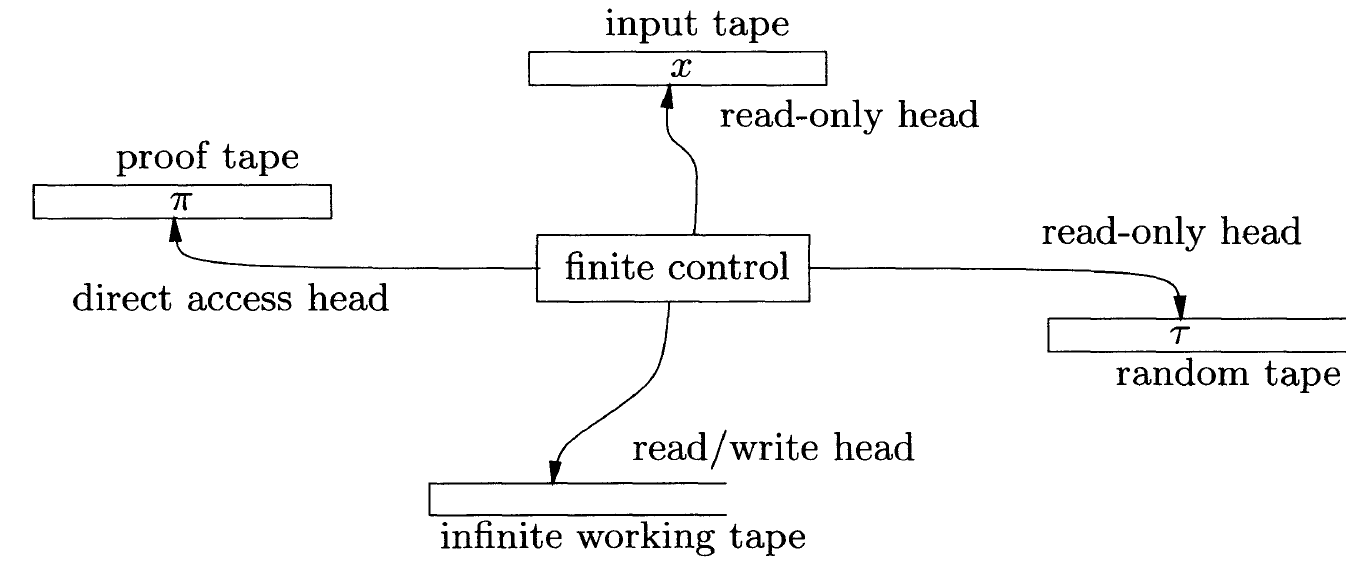
\includegraphics[width=0.6\textwidth]{images/prob-verifier.png}
    \caption{Probabilistischer Verifizierer als 4-Band-TM}
\end{figure}

\paragraph{Beschränkte Prob. Verifizierer}
Seien $r, q \in \N \mapsto \N$.
Ein \emph{$(r(n), q(n))$-beschränkter probabilistischer Verifizierer} ist ein Verifizierer,
der für jede Eingabe $x$ nur $\leq r(n)$ Zufallsbits und $\leq q(n)$ Beweisbits liest, für $|x| = n$.

$V$ \emph{akzeptiert} Sprache $L$ falls gilt:
\begin{enumerate}[label=(\roman*)]
    \item Completeness: $ \forall x \in L \cl \exists \pi \; \forall \tau \cl V(x, \tau, \pi) = \text{accept} $
    \item Soundness: $ \forall x \notin L \cl \forall \pi \cl \Pr [ V(x, \tau, \pi) = \text{accept} ] \leq \frac{1}{2} $
\end{enumerate}
wobei $ \Pr [ V(x, \tau, \pi) = \text{accept} ] = \sum_{ \tau , V(x, \tau, \pi) = \text{accept} } \Pr [\tau] $.
\\
Annahme: Zufallsbits uniform verteilt, d.h. $\Pr [\tau] = \frac{1}{2^{|\tau|}}$.

\paragraph{Beispiel (SAT)}
$(0,n)$-beschränkter Verifizierer für SAT.
Liest $m \leq n = |\Phi|$ Beweisbits und interpretiert sie als Belegung für $x_1, ..., x_m$.
Akzeptiert $x$ wenn die Belegung $\Phi$ erfüllt. Deterministisch.

$\implies$ für alle Probleme in NP existiert ein deterministischer Polynomzeit-Verifizierer
(da SAT NP-vollständig ist).

\paragraph{Beispiel (GAP$_{1-\varepsilon, 1}$(E3SAT))}
für $\varepsilon \in (0,1)$.
Eingabe $\Phi$ ist entweder erfüllbar, oder ein Teil der $m$ Klauseln sind erfüllbar
(d.h. $ Opt_{Max-E3SAT}(\Phi) < (1-\varepsilon) \cdot m$).

Ziel:
$\left( \log_{1-\varepsilon}\frac{1}{2} \cdot \log n , 3 \cdot \log_{1-\varepsilon}\frac{1}{2} \right)$%
-beschränkter prob. Verifizierer.
Logarithmisch viele Zufallsbits, konstant viele Beweisbits.

Sei $\Phi = F_1 \wedge ... \wedge F_m$ eine E3-KNF-Formel über $x_1, ..., x_d$, $d \leq 3m$.
Sei $n = |\Phi| \geq 3m$, sei $k = \lceil \log_{1-\varepsilon}\frac{1}{2} \rceil$.
$V$ wählt zufällig $k$ Klausel-Indizes (= liest $k \cdot \lceil \log_2 m \rceil$ Zufallsbits).
$V$ interpretiert $\pi_1, ..., \pi_d$ als Belegung $\alpha$ für $x_1, ..., x_d$
(wobei es nur die $\leq 3k$ Belegungen der Variablen aus $F_{i1} \wedge ... \wedge F_{ik}$ lesen muss).
$V$ prüft ob $\alpha$ diese $k$ zufälligen Klauseln erfüllt.
Wenn ja akzeptiere, sonst verwerfe.

ad (i):
$\Phi$ erfüllbar $\implies \exists$ erfüllende Belegung/Beweis $\pi$ für die $V$ immer akzeptiert.

ad (ii):
$\Phi$ nicht erfüllbar $\implies$ $\forall$ Belegung erfüllt $< (1-\varepsilon) \cdot m$ Klauseln,
d.h. $\geq \varepsilon \cdot m$ sind nicht erfüllt.
\begin{align*}
    &\Pr [ \text{eine von $\alpha$ erfüllte Klausel zu wählen } ] \geq \frac{\varepsilon \cdot m}{m} = \varepsilon \\
\implies &\Pr [ \alpha \text{ erfüllt alle } F_{i1}, ..., F_{ik} ] \leq (1-\varepsilon)^k \\
\implies &\Pr [ V \text{ reject}]
    = \Pr [ \text{mind. eine Klausel von } F_{i1}, ..., F_{ik} \text{ nicht erfüllt} ] \\
    &\geq 1 - (1-\varepsilon)^k = 1 - (1-\varepsilon)^{ \lceil \log_{1-\varepsilon}\frac{1}{2} \rceil }
    \geq \frac{1}{2} \\
\implies &\Pr [ V \text{ accept} ] \leq \frac{1}{2}
\end{align*}

$\implies$ Mit Randomisierung können wir die Anzahl notwendiger/gelesener Beweisbits reduzieren,
selbst für schwere Probleme!

\paragraph{Klasse PCP}
\emph{Probabilistically Checkable Proofs}.
Für alle $r, q \cl \N \mapsto \N$ ist
$$ PCP(r,q) = \{ L \st \text{ L is accepted by an $(r(n), q(n))$-restricted prob. verifier} \} $$

Falls $\mathcal{W}, \mathcal{V}$ Klassen nicht-fallender Funktionen sind, so gilt:
$$ PCP(\mathcal{W}, \mathcal{V}) = \bigcup_{r \in \mathcal{W} , q \in \mathcal{V}} PCP(r,q) $$

\underline{Beobachtung:}
\begin{itemize}
    \item GAP$_{1-\varepsilon, 1}$(E3SAT) $\in PCP( \bigO(\log_2n) , \bigO(1) ) $
    \item P = PCP(0,0) $\longrightarrow$ deterministisch, Beweis wird selber berechnet
    \item NP = PCP(0, poly(n)) $\longrightarrow$ vgl. Verifizierer-basierte Definition von NP
\end{itemize}

\paragraph{PCP-Theorem}
$$ NP = PCP ( \bigO(\log_2 n) , \bigO(1) ) \;
\footnote{Je nach Formulierung sind es konstant 3 Beweisbits.} $$

$\implies$ Jedes Problem in NP hat einen Beweis der sich mit konstant vielen Beweisbits
randomisiert verifizieren lässt.

\paragraph{Theorem}
GAP$_{\frac{15}{16}, 1}$(MAX-3SAT) ist NP-schwer.

\underline{Beweis:}
Zeige dass jedes $L \subseteq \Sigma^*$ in NP auf GAP$_{\frac{15}{16}, 1}$(MAX-3SAT) reduzierbar ist.
Aus dem PCP-Theorem folgt, dass es einen $( c \cdot \log_2 n , 3 )$-beschränkter prob.
Verifizierer $V$ geben muss, das $L$ akzeptiert.

\underline{Idee:}
Konstruiere für jedes $x \in \Sigma^*$ eine 3KNF-Formel $\Phi_x$ so dass gilt:
\begin{enumerate}[label=(\roman*)]
    \item $x \in L \implies \Phi_x$ erfüllbar
    \item $x \notin L \implies \forall $ Belegungen von $\Phi_x$ bleiben $\geq \frac{1}{16}$ der
        Klauseln unerfüllt
    \item $\Phi_x$ in Polynomzeit berechenbar
\end{enumerate}
Dies reduziert das Akzeptieren der Sprache $L$ auf GAP$_{\frac{15}{16}, 1}$(MAX-3SAT).

\underline{Konstruktion 3SAT-Instanz $\Phi_x$ (gegeben Eingabe $x$ und Verifizierer $V$):}
\\
Sei $\pi = \pi_1 \pi_2 ...$ das Beweisband von $V$ für Eingabe $x$.
Sei $y_i$ die Variable für Beweisbit $\pi_i$.
Konstruiere nun $\Phi_x = \bigwedge_\tau \Phi_{x, \tau}$
wobei $\tau$ über alle $n^c$ möglichen Zufallsstrings.
\footnote{Länge $c \cdot \log n \implies 2^{c \cdot \log n} = (2^{\log n})^c = n^c $
viele möglichen Strings.}

Für fixe $x, \tau$ gilt: $V$ liest (laut PCP-Theorem) drei Beweisbits $\pi_{i_1}, \pi_{i_2}, \pi_{i_3}$
und berechnet die Boolsche Funktion $f_{x, \tau}$:
%
$$ f_{x, \tau} \cl \setzeroone^3 \mapsto \underbrace{\setzeroone}_\text{reject, accept} \quad
\text{ über } Y_\tau = \{ y_{i_1}, y_{i_2}, y_{i_3} \} $$
$$ f_{x, \tau}(a_{i_1}, a_{i_2}, _{i_3}) = 1 \iff
V(x, \tau, \pi_1 \pi_2 ... a_{i_1} ... a_{i_2} ... a_{i_3} ... ) = \text{ accept } $$
%
$f_{x, \tau}$ kann eindeutig durch eine 3KNF-Formel $\Phi_{x, \tau}$
mit $\leq 2^3 = 8$ Klauseln dargestellt werden (siehe truth table).

Bestimmung von $f_{x, \tau}$: Simuliere $V(x, \tau, \tilde{\pi})$ für alle 8 Belegungen von
$\{ y_{i_1}, y_{i_2}, y_{i_3} \}$ (in Polynomzeit, da $V$ in Polynomzeit).

\underline{Bedingungen:}
\\
ad (iii): $n^c$ Teilformeln $\Phi_{x, \tau} \implies \Phi_x$ in Polynomzeit konstruierbar

ad (i): Falls $x \in L$:
$\exists \pi$ s.t. $V(x,\tau,\pi)$ = accept (per PCP-Definition)
$\implies \Phi_x$ erfüllbar

ad (ii): Falls $x \notin L$:
$V$ akzeptiert $\forall \pi$ nur $\leq \frac{1}{2}$ der $\tau$ (laut PCP). \\
$\implies \forall$ Belegung von $\Phi_x$ ist $\geq \frac{1}{2}$ der $\Phi_{x, \tau}$ unerfüllt. \\
$\implies \geq \frac{n^c}{2}$ viele $\Phi_{x, \tau}$ unerfüllt (von $\leq 8n^c$ Klauseln insgesamt in $\Phi_x$). \\
$\implies \geq \frac{1}{16}$ der Klauseln unerfüllt.
\\
\\
$\implies$ GAP$_{\frac{15}{16}, 1}$(MAX-3SAT) ist NP-schwer
\\
$\implies \not \exists \frac{16}{15}$-Approximationsalgorithmus für MAX-E3SAT (falls P $\neq$ NP).
